\documentclass{article}
\usepackage{graphicx}
\usepackage{physics}

\title{Calculus 3 notes}
\author{Joe Hollander}
\date{Summer 2024}

\begin{document}
\maketitle

\newtheorem{theorem}{Theorem}[section]

\section*{Vector Functions}
\noindent Dot product: 
\[a \cdot b = |a||b|cos(\theta).\]
Cross product:
To find the cross product of a and b find the
determinant of 3x3 matrix with unit vectors: $\mathbf{i, j, k}$
for the first row. Additionally: 
\[|a \times  b| = |a|b|sin(\theta).\]

The vector equation of a line starting at point $P$, $(a, b, c)$, 
with parralel vector $\vec{v}$, $\left\langle d, e, f\right\rangle$,
and paramater $t$:
\[
r(t) = P + t\vec{v} = 
\left\langle a + dt, b + et, c + ft\right\rangle.
\]

Given a constant point on the plane $P_0$, $(x_0,y_0,z_0)$
and a point on the plane $P$, $(x,y,z)$, 
the vector $\vec{P_0P}$ must be orthogonal to the normal vector of the plane $N$, 
$\left\langle A,B,C \right\rangle$.
Therefore, \[N \cdot \vec{P_0P} = 0, \]
and \[A(x-x_0) + B(y-y_0) + C(z-z_0) = 0.\]

Given vector function $r(t) = \left\langle f(t), g(t), h(t) \right\rangle$,
\[r'(t) = \left\langle f'(t), g'(t), h'(t) \right\rangle,\] and 
\[R(t) = \left\langle F(t), G(t), H(t) \right\rangle.\]


Length of curve from a to b is: \[\int_{a}^{b} |r'(t)| dt,\]
\[s(t) = \int_{0}^{t} |r'(x)| dx.\] An equation $y = f(x)$ can be paramaterized as
$r(t) = \left\langle t, f(t) \right\rangle$. 

The unit tangent vector: $T(t) = r'(t)/|r'(t)|$.
The principle unit normal vector: $N(t) = T'(t)/|T'(t)|$.
The binomial vector: $B = T \times N$. The osculating plane is
the one formed by $T$ and $N$. 
Curvature:
\[
\kappa(x) = |\frac{dT}{ds}| = \frac{|T'(t)|}{|r'(t)|}
= \frac{|r'(t) \times r''(t)|}{|r'(t)|^3}
\]
Torsion:
\[
\tau(x) = -N \cdot \frac{dB}{ds} 
= \frac{(r'(t) \times r''(t)) \cdot r'''(t)}{|r'(t) \cdot r''(t)|}.
\]

Working backwords from an acceleration vector, $\vec{a}$,
we can derive a position vector function of an object affected 
by gravity.
\[\vec{a} = \left\langle0, -9.8\right\rangle.\]
Given an initial velocity vector, $\vec{v_0}$ with speed, $s$,
and angle, $\alpha$: 
\[\vec{v_0} = \left\langle s\cos(\alpha), s\sin(\alpha)\right\rangle,\]
\[v(t) = \left\langle s\cos(\alpha), -9.8t + s\sin(\alpha)\right\rangle,\]
and
\[r(t) = \left\langle s\cos(\alpha)t, -4.9t^2 + s\sin(\alpha)t\right\rangle,\]
\[x = s\cos(\alpha)t, y = -4.9t^2 + s\sin(\alpha)t\].

\section*{Partial Derivatives}\

Domain for a function of two variables can be written as: 
\[D = \{(x,y)\:|\: x + y != 2, xy < -1\}.\]
Similar to contour drawings on maps, level curves of a function $f$ of two variables
are the curves with equations $f(x,y) = k$ where $k$ is a constant. 
\begin{center}
    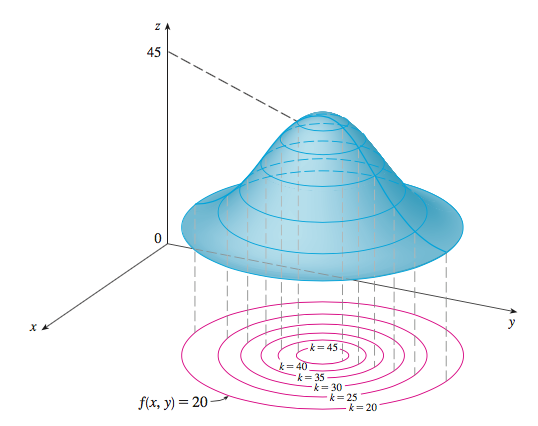
\includegraphics[width=12cm,height=12cm, keepaspectratio]{LevelCurves.png}
\end{center}
Functions of three variables are the same as functions of two variables and
functions of multiple variables can be packaged into a function of one vector
variable. 

For multivariable limits, the notation is:
\[\lim_{(x,y)\to (a,b)}f(x,y) = L.\]
Since the limit of a multi variable function can be approached from any way,
the definition of what makes a limit not exist has to be redefined. If 
$f(x,y) \to L_1$ as $(x,y) \to (a,b)$ along a path $C_1$ and $f(x,y) \to L_2$ as
$(x,y) \to (a,b)$ along a path $C_2$ and $L_1 \neq L_2$, then $\lim_{(x,y)\to (a,b)}f(x,y)$
does not exist. The easiest paths to evaluate are often the x and y-axis. 
If evaluating on the x-axis (or y-axis) substitute in $y=b$ (or $x=a$) and then solve
\[\lim_{(x,y) \to (a, b)} f(x,b),\] or \[\lim_{(x,y) \to (a, b)} f(a,y).\] 
Substituting in $y = mx$ is also an easy path to evaluate. A polynomial function of two variables
is in the form: \[f(x,y) = cx^n y^n.\] A rational polynomial is the ratio of two polynomials.
Since a polynomial is continous everywhere, a polynomial $p$ has the property:
\[\lim_{(x,y) \to (a,b)} p(x,y) = p(a,b).\]
Similarly a rational function $q$ has the same property provided $r(a,b) \neq 0$:
\[\lim_{(x,y) \to (a,b)} q(x,y) = \frac{p(a,b)}{r(a,b)} = q(a,b).\]
Squeeze theorem applies to multivariable functions also. Additionally,
the epsilon-delta definition of a limit is useful in proving that the limit is a value.
The definition states that for every $\epsilon > 0$ there exists a $\delta > 0$. 
$\delta$ bounds the domain such that:
\[0 < \sqrt{(x-a)^2 + (y-b)^2} < \delta,\]
and $\epsilon$ bounds the range such that: \[|f(x,y) - L| < \epsilon.\]
It's often easiest to start with the epsilon inequality first,
and finding a relation between delta and epsilon such as $\delta = \epsilon/3$
completes the proof. The epsilon-delta definition extends to vector functions:
\[0 < |\vec{x} - \vec{a}| < \delta, \] and
\[|f(\vec{x}) - L| < \epsilon.\]

A multivariable function is defined as continous if
\[\lim{(x,y) \to (a,b) f(x,y) = f(a,b)}.\] 
If two functions $f$ and $g$ are continuous then their composition function
$h = f \: \circ g = f(g(x,y))$ is also continous. Fix $y=b$ so that $g(x)=f(x,b)$.
The derivative of $f$ with respect to $x$ at $a$ is denoted by:
\[g'(a) = f_x(a,b).\] Therefore, the limit definition becomes:
\[f_x(a,b) = \lim_{h \to 0}\frac{f(a+h,b) - f(a,b)}{h},\]
or \[f_y(a,b) = \lim_{h \to 0}\frac{f(a,b+h) - f(a,b)}{h}.\]

\noindent Visually: 
\begin{center}
    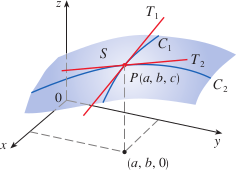
\includegraphics[width=12cm,height=12cm, keepaspectratio]{PartialDerivative.png}
\end{center}

When implicity differentiating equations with respect to $x$ such as:
\[x^3 + y^3 + z^3 + 6xyz = 0,\] where $z = f(x,y)$. Treat $y$ as a constant and $z$
as a function of $x$. Therefore, the derivative would be:
\[3x^2 + 3z^2\pdv{z}{x} + 6yz + 6xy\pdv{z}{x} = 0.\]
Partial derivatives of functions of three variables are the same. Second order
partial derivatives are denoted as:
\[(f_x)_x = \pdv[2]{f}{x},\]
and partial derivatives of order $n$ are denoted as:
\[\pdv[n]{f}{x}.\]
Clairaut's theorem states that if $f$ is defined on a domain disk $D$ that contains
the point $(a,b)$ then
\[f_{xy}(a,b) = f_{yx}(a,b).\]

Tangent plane contains both tangent lines from the derivative with respect to $x$
and the derivative with respect to $y$.  
\begin{center}
    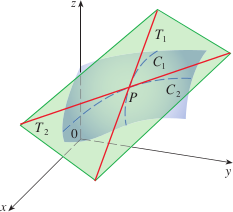
\includegraphics[width=12cm,height=12cm, keepaspectratio]{TangentPlane.png}
\end{center}

Another equation of a plane is:
\[z-z_0=a(x-x_0) + b(y-y_0),\]
where $a = -A/C$ and $b = -B/C$. Remember the normal vector:
 $N = \left\langle A, B, C \right\rangle.$ Since setting $y=y_0$ or
 $x=x_0$ represents the tangent line in the $x$ or $y$ plane respectively, 
 the equation of a tangent plane given the derivatives with respect to $x$ and $y$
 at the point $(x_0, y_0, z_0)$ is: 
 \[z-z_0 = f_x(x_0, y_0)(x-x_0) + f_y(x_0, y_0)(y-y_0).\]
 This equation can be used to 
 approximate $z$ close to $(x_0, y_0)$. Specifically, this linear function:
 \[L(x,y) = f(a,b) +f_x(a,b)(x-a)+f_y(a,b)(y-b),\] is called
 the linearization for $f$ at $(a,b).$ A two variable function is
considered differentiable at $(a,b)$ if:
\[\Delta z = f_x(a,b)\Delta x + f_y(a,b)\Delta y + \epsilon_1\Delta x + \epsilon_2\Delta y,\]
where $\epsilon_1$ and $\epsilon_2$ are functions of $\Delta x$ and $\Delta y$
such that $\epsilon_1$ and $\epsilon_2 \to 0$ as $(\Delta x,\Delta y) \to (0,0).$
Rephrased, if the partial derivatives exist and are continous at $(a,b)$,
then the function is differentiable at $(a,b)$. 

$\Delta z$ is the 
actual change in $z$, while $dz$ is the linear approximation of the change in $z$:
\[dz = \pdv{z}{x}dx + \pdv{z}{y}dy.\]

One of the chain rules for multivariable functions:
\[\dv{z}{t} = \pdv{z}{x}\dv{x}{t} + \pdv{z}{y}\dv{y}{t}.\]
When $x$ and $y$ are functions of two variables $s$ and $t$, 
\[\dv{z}{s} = \pdv{z}{x}\pdv{x}{s} + \pdv{z}{y}\pdv{y}{s},\]
\[\dv{z}{t} = \pdv{z}{x}\pdv{x}{t} + \pdv{z}{y}\pdv{y}{t}.\]
Finding $y'$ from the implicitly defined equation:
\[x^3 + y^3 = 6xy.\]
We can write this equation as:
\[F(x,y) = x^3 + y^3 - 6xy = 0.\]
Knowing that $y$ can be written as a function of $x$ and that 
$F(x,y) = 0$, we can rewrite 
\[\pdv{F}{x} + \pdv{F}{y}\dv{y}{x} = 0,\]
as \[\dv{y}{x} = -\frac{F_x}{F_y}.\]
Therefore, in the above equation 
\[y' = -\frac{F_x}{F_y} = -\frac{x^2 - 2y}{y^2 -2x}.\]
Extending this result, for the equation
\[F(x,y,z)=F(x,y,f(x,y))=0,\]
\[\pdv{z}{x} = -\frac{F_x}{F_z},\] and
\[\pdv{z}{y} = -\frac{F_y}{F_z}.\]

The directional derivative of $f$ at $(x_0, y_0)$ in the direction
of a unit vector $\mathbf{u} = \left\langle a,b \right\rangle$:
\[D_uf(x_0,y_0) = \lim_{h \to 0}\frac{f(x_0 + ha, y_0 + hb) - f(x_0,y_0)}{h}.\]
If $f$ is a directional function of $x$ and $y$, then $f$ has a directional
derivative in the direction of the unit vector $\mathbf{u} = \left\langle a,b \right\rangle$
and \[D_uf(x,y) = f_x(x,y)a + f_y(x,y)b
= \left\langle f_x(x,y),f_y(x,y) \right\rangle \cdot \mathbf{u}
.\]
$\left\langle f_x(x,y),f_y(x,y) \right\rangle$ is called the gradient vector of
$f$ and is also denoted by $\nabla f$. Also defined by:
\[\nabla f(x,y) = \pdv{f}{x}\mathbf{i} + \pdv{f}{y}\mathbf{j}.\]
Therefore, the directional derivative can be written as:
\[D_uf(x,y)=\nabla f(x,y) \cdot \mathbf{u}.\]

The maximum of the directional derivative 
$D_uf(\mathbf{x})$ is $|\nabla f(\mathbf{x})|)$, and it occurs when
$\mathbf{u}$ has the same direction as the gradient vector $\nabla f(\mathbf{x})$.

Given a level surface $F(x,y,z) = k$, the gradient vector $\nabla F$
is perpendicular to the surface, and therefore, the tangent plane to the surface
can be represented by the point and the gradient vector of that point.
Using the standard equation of a plane:
\[F_x(x_0,y_0,z_0)(x-x_0)+F_y(x_0,y_0,z_0)(y-y_0)+F_z(x_0,y_0,z_0)(z-z_0)=0.\]
The normal line is the line perpendicular to the surface at point $(x_0,y_0,z_0)$,
and therefore, its symmetric equations are:
\[\frac{x-x_0}{F_x(x_0,y_0,z_0)} = \frac{y-y_0}{F_y(x_0,y_0,z_0)}
 = \frac{z-z_0}{F_z(x_0,y_0,z_0)}.\]
For an equation defined by $z=f(x,y)$, we can rewrite the equation as:
\[F(x,y,z) = f(x,y) - z = 0.\] In this situation
\[F_x(x_0,y_0,z_0) = f_x(x_0,y_0),\]
\[F_y(x_0,y_0,z_0) = f_y(x_0,y_0),\]
\[F_z(x_0,y_0,z_0) = -1.\]





\end{document}